\documentclass{article}
\usepackage{graphicx}
\usepackage{amsmath}
\usepackage{hyperref}
\usepackage{float}

\begin{document}

\title{Solutions to hw5 homework on Convex Optimization https://web.stanford.edu/class/ee364a/homework.html}
\author{Andrei Keino}
\maketitle

% https://web.stanford.edu/class/ee364a/homework.html
% 6.3, 6.8a-b, A5.4, A12.6, A14.8, A17.9

% 5.17 - p. 278
% Robust linear programming cvxbook p. 157
% duality - from p.215

\section*{5.17}
Robust linear programming with polyhedral uncertainty. Consider the robust LP:

\begin{align*}
&\text{minimize } && c^T x \\
&\text{subject to } &&\sup_{a \in P_i} a^T x \leq b_i, \; i = 1, ... , m\\
\end{align*} 

with variable $x \in R^n, $ where
$P_i = \{a: \; C_i a \preceq d_i \}.$ The problem data are $a \in R^n,$ $C_i \in R^{m_i \times n}, $ $d_i \in R^{m_i}, $ and $b \in R^m.$ We asume the polyhedra $P_i$ are nonempty. Show that this problem is equivalent to the LP:

\begin{align*}
&\text{minimize } && c^T x \\
&\text{subject to } &&d_i^T z_i \leq b_i,
\; i = 1, ... , m\\
& && C_i z_i = x, \; i = 1, ... , m\\
& && z_i \succeq 0, \; i = 1, ... , m\\
\end{align*} 
with variables $x \in R^n, $ 
$z_i \in R^{m_i}, \; i = 1, ... , m.$ 
Hint: find the dual of the problem of maximizing 
$a_i^T x$ over $a_i \in P_i$ (with variable $a_i$).\\

Solution: \\

The problem of maximizing 
$a_i^T x$ over $a_i \in P_i$ (with variable $a_i$) is:

\begin{align*}
&\text{maximize } && a_i^T x \\
&\text{subject to } &&a_i \in P_i, \text{where } 
P_i = \{a: \; C_i a \preceq d_i \}\\
\end{align*} 

or 

\begin{align*}
&\text{minimize } && - a_i^T x \\
&\text{subject to } &&C_i a_i \preceq d_i \\
\end{align*} 

The Lagrange dual of this problem is:

\begin{align*}
&\text{minimize } && \sum_{i = 1}^{m} \lambda_i d_i \\
&\text{subject to } 
&& C_i \lambda_i = x \\
& &&\lambda_i \succeq 0\\
\end{align*} 

The optimal value of this problem is less or equal to $b_i$, so we have the equivalent problem to our LP:

\begin{align*}
&\text{minimize } && c^T x \\
&\text{subject to } &&d_i^T \lambda_i \leq b_i,
\; i = 1, ... , m\\
& && C_i \lambda_i = x, \; i = 1, ... , m\\
& && \lambda_i \succeq 0, \; i = 1, ... , m\\
\end{align*} 

\section*{5.40}
% ex. 5.40 - p. 286
% ex. 5.10 - p. 276
% paragraph 7.5 - p. 384
 
E - optimal experiment design. A variation on two optimal experiment design problems of exercise 5.10
is the E - optimal design problem:

\begin{align*}
&\text{minimize } && \lambda_{max}
(\sum_{i = 1}^p x_i v_i v_i^T)^{-1} \\
&\text{subject to } 
&&x \succeq 0, \; \boldsymbol{1}^T x = 1\\
\end{align*} 

(See also \S 7.5.) Derive a dual for this problem first by reformulating it as: 
 
\begin{align*}
&\text{minimize } && 1 / t \\
&\text{subject to } 
&& \sum_{i = 1}^p x_i v_i v_i^T
\succeq t \boldsymbol{I} \\
& &&x \succeq 0, \; \boldsymbol{1}^T x = 1
\end{align*} 

with variables $t \in R,$ $x \in R^p$ and domain 
$R_{++} \times R^p,$ and applying Lagrange duality. Simplify the dual problem as much as you can.

Solution:
Let us introduce a variable $t  \in R_{++}.$ Then for a matrix $A,$ inequality 
$\lambda_{max}(A^{-1})  \leq 1 / t$ means $A^{-1} \preceq \frac{1}{t}\boldmath{I},$ or 
$A \preceq t \boldmath{I}.$ Setting $A$ to 
$\sum_{i = 1}^p x_i v_i v_i^T$ we get a problem:

\begin{align*}
&\text{minimize } && 1 / t \\
&\text{subject to } 
&& \sum_{i = 1}^p x_i v_i v_i^T
\succeq t \boldsymbol{I} \\
& &&x \succeq 0, \; \boldsymbol{1}^T x = 1
\end{align*} 

% Entropy maximization - p.222 
% Generalized inequalities - p. 264
% Example 5.11 Lagrange dual of semidefinite program - p. 265

% Lagrange function - https://math.stackexchange.com/questions/462896/is-positive-semidefinite-matrix-same-as-positive-number-in-convex-optimisation

% https://en.wikipedia.org/wiki/Semidefinite_programming

% Semidefinite programming - p. 168

The Lagrangian is: 

$$
L(x, t, Z, z) = 1 / t - 
tr(Z (\sum_{i = 1}^p x_i v_i v_i^T - t \boldsymbol{I})) - z^T x + 
\nu (\boldsymbol{1}^T x - 1) \\ 
= 1 / t + t \, tr(Z) + 
\sum_{i = 1}^p x_i 
(-v_i^T Z v_i - z_i + \nu) - \nu
$$
the infimum of x is bounded below only if 
$-v_i^T Z v_i - z_i + \nu = 0.$ The 

$$
inf_\nu 1/t  + t \, tr(Z) = 
\begin{cases}
2 \sqrt{tr(Z)}, & Z \succeq 0 \\
- \infty, & \text{otherwise}
\end{cases}
$$
the dual function is 

$$
L(Z, z, \nu) = 
\begin{cases}
2 \sqrt{tr(Z)} - \nu, & Z \succeq 0, \,  
-v_i^T Z v_i - z_i + \nu = 0,\\
- \infty, & \text{otherwise}
\end{cases}
$$

The dual problem:

\begin{align*}
&\text{maximize } && 2\sqrt{tr(Z)} - \nu \\
&\text{subject to } 
&& v_i^T Z v_i + z_i \leq 0, 
\; i = 1, ..., p  \\
& &&Z \succeq 0, \, \nu \geq 0\\
\end{align*} 

We can define $W = (1 / \nu)Z$
\begin{align*}
&\text{maximize } && 2\sqrt{\nu}\sqrt{tr(W)} - \nu \\
&\text{subject to } 
&& v_i^T W v_i \leq 1, 
\; i = 1, ..., p  \\
& &&W \succeq 0, \, \nu \geq 0
\end{align*} 

Maximizing over $\nu$ we get $\nu = tr(W), $
so the problem is:

\begin{align*}
&\text{maximize } && tr(W) \\
&\text{subject to } 
&& v_i^T W v_i \leq 1, 
\; i = 1, ..., p  \\
& &&W \succeq 0\\
\end{align*} 

\section*{6.3}
% p. 344

%LPs, QPs, SOCPs, or SDPs

% LP - Linear optimization problems - p. 146
% QP - Quadratic optimization problems - p.152

% Geometric programming - p. 160
% SDP - Semidefinite programming - p. 168
% SOCP - Second-order cone programming - p. 156
% QCQP - p. 153
% GP geometric program - p. 161

Formulate the following approximation problems as LPs, QPs, SOCPs, or SDPs. The
problem data are $A \in R^{n \times m}$ and 
$b \in R^m.$ The rows of $A$ are denoted $a_i^T.$

(a) Deadzone-linear penalty approximation: minimize $\sum_{i = 1}^m \phi(a_i^T x - b_i),$ where 

$$
\phi(u) = 
\begin{cases}
0, & |u| \leq a \\
|u| - a, & |u| > a
\end{cases}
$$
where $a > 0.$

(b) Log-barrier penalty approximation: 
minimize $\sum_{i = 1}^m \phi(a_i^T x - b_i),$ where 

$$
\phi(u) = 
\begin{cases}
- a^2 log(1 - (u / a)^2), & |u| < a \\
\infty, & |u| \geq a
\end{cases}
$$
with $a > 0.$

(c) Huber penalty approximation: minimize 
 $\sum_{i = 1}^m \phi(a_i^T x - b_i),$ where 

$$
\phi(u) = 
\begin{cases}
u^2, & |u| \leq M \\
M(2|u| - M), & |u| > M
\end{cases}
$$
with $M > 0.$

(d) Log-Chebyshev approximation: minimize
$max_{i = 1, ..., m} 
|log(a_i^T x) - log(b_i)|.$ We assume 
$b \succ 0.$ An equivalent convex from is

\begin{align*}
&\text{minimize } && t \\
&\text{subject to } 
&& 1/t \leq a_i^Tx/b_i \leq t, \, i = 1 ,..., m\\
\end{align*} 
with variables $x \in R^n$ and $t \in R$ and domain $R^n \times R_{++}.$

(e) Minimizing the sum of the largest k residuals:

\begin{align*}
&\text{minimize } && 
\sum_{i = 1}^k |r|_{[i]} \\
&\text{subject to } 
&& r = Ax - b\\
\end{align*} 

where $|r|_{[1]} \geq |r|_{[2]} \geq ,..., 
\geq |r|_{[m]}$ are the numbers 
$|r_1|, |r_2|, ... , |r_m| $ sorted in decreasing order. (For $k = 1$ this reduces to $l_\infty$ - norm approximation; for $k = m$ this reduces to $l_1$ norm approximation.) Hint: See exercise 5.19.

Solution:

(a) Introduce the variable $y \in R^m$ so that 
$|a_i^T x - b_i| \leq |a + y_i|, \, y_i \geq 0$

then we have equivalent problem:
\begin{align*}
&\text{minimize } && \boldsymbol{1}^Ty \\
&\text{subject to } 
&& - y - a \boldsymbol{1} \preceq A x - b 
\preceq y + a \boldsymbol{1} \\
& && y \ \succeq 0\\
\end{align*}

(b)

Introduce the variable $y = Ax - b, $ 
$t_i \leq (1 - y_i / a)(1 + y_i + a)$, and add inequality $-a \leq y_i \leq a$ this problem will transform to:

\begin{align*}
&\text{maximize } && \prod_{i = 1}^m t_i^2 \\
&\text{subject to } && y = A x - b \\
& && t_i \leq (1 - y_i / a)(1 + y_i / a),
\, i = 1, ..., m\\
& && -1 \leq y_i / a \leq 1, \, i = 1, ..., m\\
\end{align*}
with variables $t, y \in R^m,$ $x \in R^n.$
Next assume that $m = 2^k.$ It can be done without loss of generality, as in other case we always can add missing components of $y_i$ as unity values ($a_i = 0$ and 
$b_i = - 1$). Lets transform this problem for $m = 4.$

\begin{align*}
&\text{maximize } && (t_1 t_2 t_3 t_4)^2 \\
&\text{subject to } && y = A x - b \\
& && t_i \leq (1 - y_i / a)(1 + y_i / a),
\, i = 1, ..., m\\
& && -1 \leq y_i / a \leq 1, \, i = 1, ..., m\\
\end{align*}

this problem is equivalent to:

\begin{align*}
&\text{maximize } && z_1 z_2 \\
&\text{subject to } && \\
& && z_1^2 \leq t_1 t_2 \\
& && z_2^2 \leq t_3 t_4 \\
& && y = A x - b \\
& && t_i \leq (1 - y_i / a)(1 + y_i / a),
\, i = 1, ..., m\\
& && -1 \leq y_i / a \leq 1, \, i = 1, ..., m\\
\end{align*}

and also as:

\begin{align*}
&\text{maximize } && z \\
&\text{subject to } && \\
& && z^2 \leq z_1 z_2\\
& && z_1^2 \leq t_1 t_2 \\
& && z_2^2 \leq t_3 t_4 \\
& && y = A x - b \\
& && t_i \leq (1 - y_i / a)(1 + y_i / a),
\, i = 1, ..., m\\
& && -1 \leq y_i / a \leq 1, \, i = 1, ..., m\\
\end{align*}

as it is easy to show that $x^T x \leq yz$ where 
$x \in R^n, $ $y, z \in R_+$ is equivalent to:

$$
\left\lVert
\begin{bmatrix}
	x \\ y - z\\
\end{bmatrix}
\right\rVert_2 \leq y + z
$$

overriding the first three inequalities with their norm analogue we have:

\begin{align*}
&\text{minimize } && - z \\
&\text{subject to } && \\
& && 
\left\lVert
\begin{bmatrix}
z \\ z_1 - z_2\\
\end{bmatrix}
\right\rVert_2 \leq z_1 + z_2\\
& && \left\lVert
\begin{bmatrix}
z_1 \\ t_1 - t_2\\
\end{bmatrix}
\right\rVert_2 \leq t_1 + t_2\\
& && \left\lVert
\begin{bmatrix}
z_2 \\ t_3 - t_4\\
\end{bmatrix}
\right\rVert_2 \leq t_3 + t_4\\
& && y = A x - b \\
& && t_i \leq (1 - y_i / a)(1 + y_i / a),
\, i = 1, ..., m\\
& && -1 \leq y_i / a \leq 1, \, i = 1, ..., m\\
\end{align*}

which is Second Order Cone Program (SOCP). \\

(c)\\
Lets show that this problem is equivalent to QP:
\begin{align*}
&\text{minimize } && 
\sum_{i = 1}^m(u_i^2 + 2 M v_i) \\
&\text{subject to } && 
-u - v \preceq Ax - b \preceq u + v\\
& && 0 \preceq u \preceq M \boldsymbol{1}\\
& && v \succeq 0
\end{align*}
Proof: Lets fix $x$ in our QP. For the optimum point we must have \\
$u_i + v_i = |a_i^T x - b_i|.$
In other case, if 
$u_i + v_i > |a_i^T x b_i|$ and 
$0 \leq u_i \leq M$ and $v_i \geq 0, $ then as $u_i$ and $v_i$ are not both zero, we can decrease $u_i$ and/or $v_i$ without violating the constraints and the objective will be decreased also. So, at the optimum we have:
$$ v_i = |a_i^T x - b_i| - u_i$$ 
Eliminating $v_i$ yields equivalent problem:
\begin{align*}
&\text{minimize } && 
\sum_{i = 1}^m
(u_i^2 - 2 M u_i + 2 M |a_i^T x - b_i|) \\
&\text{subject to }
&& 0 \preceq u_i \preceq 
min(M, \, |a_i^T x - b_i|)\\
\end{align*}
It $M > |a_i^T x - b_i|$ the optimal choice for 
$u_i$ is $|a_i^T x - b_i|.$ In this case the objective function reduces to 
$|a_i^T x - b_i|^2.$ Otherwise the optimal choice for $u_i$ is $M,$ and the objective function reduces to $2 M |a_i^T x - b_i| - M^2.$ So, we conclude that with $\phi(a_i^T x - b_i)$ these problems are equivalent.\\
(c) The constraint $ta_i^Tx \geq b_i,$ $t \geq 0,$
$a_i^T x \geq 0$ can be formulated as an LMI 
$$
\begin{bmatrix}
	t & \sqrt{b_i}\\
	\sqrt{b_i} & a_i^Tx\\
\end{bmatrix} \succeq 0
$$

or as follows:

$$
\left\Vert
\begin{bmatrix}
 2\sqrt{b_i}\\
t - a_i^Tx\\
\end{bmatrix} 
\right\Vert_2 \leq t + a_i^Tx
$$

% 5.19 - p. 278
% this - p.345
(e) As in exercise 5.19, we have a problem:

\begin{align*}
&\text{minimize } && 
kt + \boldsymbol{1}z \\
&\text{subject to }
&& - t \boldsymbol{1} - z \preceq Ax - b \preceq 
t \boldsymbol{1} +z \\
& && z \succeq 0
\end{align*}
where $x \in R^n,$ $t \in R,$ $z \in R^m$

\section*{6.8 a - b} % p. 346
Formulate the following robust approximation problems as LPs, QPs, SOCPs, or SDPs. For each subproblem, consider the $l_1 - ,$  $l_2 - ,$ and the $l_{\infty} - $ norms.

(a) Stochastic robust approximation with a finite set of parameter values, i.e., the sum of - norms problem

\begin{align*}
&\text{minimize } && 
\sum_{i = 1}^k
p_i\left\lVert A_ix - b\right\lVert  \\
\end{align*}
where $p \succeq 0$ and $\boldsymbol{1}^Tp = 1.$ 
(See \S6.4.1.)

(b) Worst-case robust approximation with coefficient bounds:
\begin{align*}
&\text{minimize } && 
\sup_{A \in \mathcal{A}}
\left\lVert Ax - b\right\lVert  \\
\end{align*}
where $\mathcal{A} = \{A \in R^{m\times n} | 
l_{ij} \leq a_{ij} \leq u_{ij}, i = 1, ..., m, 
	j = 1, ... , n\}.$ Here the uncertainty set is described by giving upper and lower bounds for the
components of $A$. We assume $l_{ij} < u_{ij}.$ \\

Solution:\\
(a) $l_1$ norm: Introduce a slack variable $y: $ 
$|y_i| \succeq |A_i x - b|.$ We have LP:

\begin{align*}
&\text{minimize } && 
p^Ty \\
&\text{subject to }
&& -y_i \preceq A_ix - b \preceq y_i \\
\end{align*}

$l_2$ norm: Introduce a slack variable $y: $ 
$y_i \succeq ||A_i x - b||_2.$ We have SOCP:

\begin{align*}
&\text{minimize } && 
p^Ty \\
&\text{subject to }
&& ||A_ix - b|| \preceq y_i \\
\end{align*}

$l_{\infty}$ norm:  We have LP:

\begin{align*}
&\text{minimize } && 
p^Ty \\
&\text{subject to }
&& -y_i \boldsymbol{1} \preceq A_ix - b 
\preceq y_i  \boldsymbol{1}\\
\end{align*}
\\
(b) 
$$
\sup_{l_{ij} \leq a_{ij} \leq u_{ij}} |a_i^Tx - b_i| = 
\sup_{l_{ij} \leq a_{ij} \leq u_{ij}} 
max(- a_i^Tx + b_i, a_i^Tx - b_i) = 
max(\sup_{l_{ij} \leq a_{ij} \leq u_{ij}} - a_i^Tx + b_i, 
\sup_{l_{ij} \leq a_{ij} \leq u_{ij}} a_i^Tx - b_i)
$$

$$
\sup_{l_{ij} \leq a_{ij} \leq u_{ij}} - a_i^Tx + b_i = 
\overline - a_i^T x + b_i + v_i^T |x|
$$
where 
$\overline a_{ij} = (u_{ij} + l_{ij}) / 2, $ $v_{ij} = (u_{ij} - l_{ij}) / 2$ and 

$$
\sup_{l_{ij} \leq a_{ij} \leq u_{ij}} a_i^Tx - b_i = 
\overline a_i^T x - b_i + v_i^T |x|
$$

Therefore 

$$
\sup_{l_{ij} \leq a_{ij} \leq u_{ij}} |a_i^Tx - b_i| = 
\overline |a_i^T x - b_i| + v_i^T |x|
$$
\\

(a) $l_1$ norm.

\begin{align*}
&\text{minimize } && 
\sum_{i = 1}^m (|\overline a_i x - b_i| + v_i^T |x|) \\
\end{align*}

Introducing slack variables 
$y:$ $|y_i| \geq |\overline a_i x - b_i|$
and 
$w:$ $|w_i| \geq |x_i|$
we have LP:

\begin{align*}
&\text{minimize } && 
\boldsymbol{1}^T(y + Vw)  \\
&\text{subject to } 
&& - y \preceq \overline Ax - b \preceq y\\
& && -w \preceq x \preceq w
\end{align*}
\\
$l_2$ norm.

\begin{align*}
&\text{minimize } && 
\sum_{i = 1}^m (|\overline a_i x - b_i| + v_i^T |x|)^2 \\
\end{align*}

introduce the same slack variables and variable $y, w$ and the new variable  $t:$ 
$t \leq ||y + Vw||_2$ we have SOCP:

\begin{align*}
&\text{minimize } && 
t \\
&\text{subject to } 
&& - y \preceq \overline Ax - b \preceq y\\
& && -w \preceq x \preceq w \\
& && t \geq ||y + Vw||_2
\end{align*}
\\

$l_{\infty}$ norm:

\begin{align*}
&\text{minimize } && 
\max_{i = 1, ..., m} (|\overline a_i x - b_i| + v_i^T |x|)^2 \\
\end{align*}

this can be expressed as LP:

\begin{align*}
&\text{minimize } && 
t \\
&\text{subject to } 
&& - y \preceq \overline Ax - b \preceq y\\
& && -w \preceq x \preceq w \\
& && - t\boldsymbol{1} \preceq y + Vw \preceq t\boldsymbol{1}
\end{align*}

\section*{A5.4} % p. 58
Penalty function approximation. We consider the approximation problem
\begin{align*}
&\text{minimize } && 
\phi(Ax + b) \\
\end{align*}
where $a \in R^m\times n,$ $b \ in R^m,$ the variable is 
$x \in R^n,$ and $\phi : $ $R^m \rightarrow R$ is a convex penalty function that measures the quality of the approximation
$Ax \approx b.$ We will consider the following
choices of penalty function: \\

(a) Euclidean norm.
$$
\phi(y) = ||y||_2 = (\sum_{k=1}^m y_k^2)^{1/2}
$$
\\

(b) $l_1$ -  norm:
$$
\phi(y) = ||y||_1 = \sum_{k=1}^m |y_k|
$$
\\

(c) Sum of the largest $m/2$ absolute values:
$$
\phi(y) = \sum_{k=1}^{m/2} |y_{[k]}|
$$
where $y_{[1]}, y_{[2]},...$ denote the the absolute values of the components of $y$ sorted in the decreasing order.
\\

(d) A piecewise-linear penalty.
$$
\phi(y) = \sum_{k = 1}^m h(y_k), \quad 
h(u) = \begin{cases}
0, &|u| \leq 0.2\\
|u| - 0.2, &0.2 \leq |u| \leq 0.3 \\
2 |u| - 0.5, &|u| \geq 0.3 \\
\end{cases}
$$
\\

(e) Huber penalty. 

$$
\phi(y) = \sum_{k = 1}^m h(y_k), \quad 
h(u) = \begin{cases}
u^2, &|u| \leq M\\
M(2|u| - M), &|u| \geq M\\
\end{cases}
$$
with $M = 0.2$
\\

(f) Log-barrier penalty. 
$$
\phi(y) = \sum_{k = 1}^m h(y_k), \quad 
h(u) = - log(1 - u^2), \quad
\boldsymbol{dom} \;h = \{u\,| \; |u| < 1.\}
$$
with $M = 0.2$
\\

Here is the problem. Generate data A and b as follows:

\begin{verbatim}
m = 200;
n = 100;
A = randn(m,n);
b = randn(m,1);
b = b/(1.01*max(abs(b)));
\end{verbatim}

(The normalization of b ensures that the domain of $\phi(Ax - b)$
is nonempty if we use the log-barrier penalty.) To compare the results, plot a histogram of the vector of residuals
$y = Ax - b$ for each
of the solutions $x$, using the Matlab command
\begin{verbatim}
hist(A*x-b,m/2);
\end{verbatim}

Some additional hints and remarks for the individual problems:\\
(a) This problem can be solved using least-squares \verb|(x=A\b).| \\
(b) Use the CVX function \verb|norm(y,1).|\\
(c) Use the CVX function \verb|norm_largest().| \\
(d) Use CVX, with the overloaded \verb|max(),| \verb|abs(),| and \verb|sum()|  functions.\\
(e) Use the CVX function \verb|huber().|\\
(f) The current version of CVX handles the logarithm using an iterative procedure, which is slow
and not entirely reliable. However, you can reformulate this problem as
\begin{align*}
&\text{maximize } && 
\prod_{k = 1}^m ((1 - (Ax - b)_k)(1 + (Ax - b)_k)))^{1 / 2m},  \\
\end{align*}
and use the CVX function \verb|geo_mean().| \\

Solution:

(a)\\
Matlab code:
\begin{verbatim}
m = 200;
n = 100;
A = randn(m,n);
b = randn(m,1);
b = b/(1.01*max(abs(b)));

x = A \ b;

hist(A*x-b,m/2);
saveas(gcf,'C:/! Convex_Optimization/homework_solutions/part_1/hw5/A_5_4_a.png')
\end{verbatim}

\begin{figure}[H]
	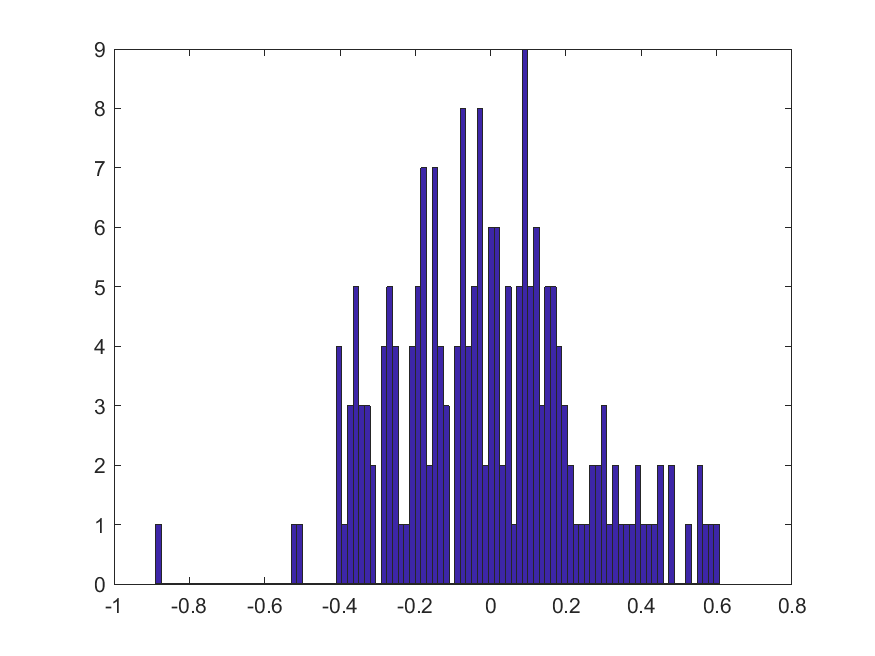
\includegraphics[width=\linewidth]{A_5_4_a.png}
	\caption{Euclidean norm}
\end{figure}

(b)\\
Matlab code:

\begin{verbatim}
m = 200;
n = 100;
A = randn(m,n);
b = randn(m,1);
b = b/(1.01*max(abs(b)));

cvx_begin
variable x(n);
variable y(m);
minimize norm(A * x - b, 1)
cvx_end

hist(A*x-b,m/2);
saveas(gcf,'C:/! Convex_Optimization/homework_solutions/part_1/hw5/A_5_4_b.png')
\end{verbatim}

\begin{figure}[H]
	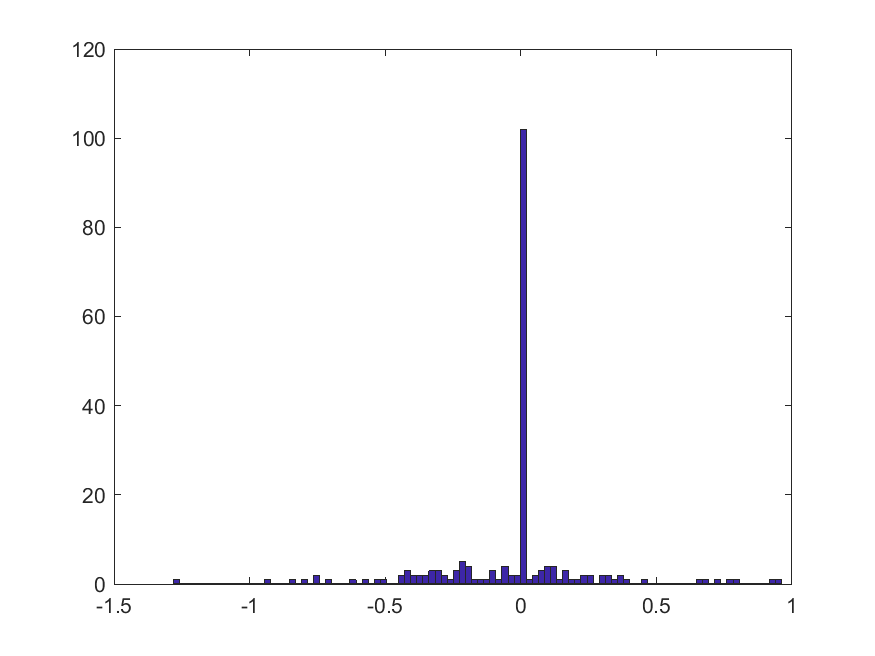
\includegraphics[width=\linewidth]{A_5_4_b.png}
	\caption{$l_1-$norm.}
\end{figure}

(c)\\
Matlab code:

\begin{verbatim}
m = 200;
n = 100;
A = randn(m,n);
b = randn(m,1);
b = b/(1.01*max(abs(b)));

cvx_begin
variable x(n);
variable y(m);
minimize norm_largest(A * x - b, floor(m / 2))
cvx_end

hist(A*x-b,m/2);
saveas(gcf,'C:/! Convex_Optimization/homework_solutions/part_1/hw5/A_5_4_c.png')
\end{verbatim}

\begin{figure}[H]
	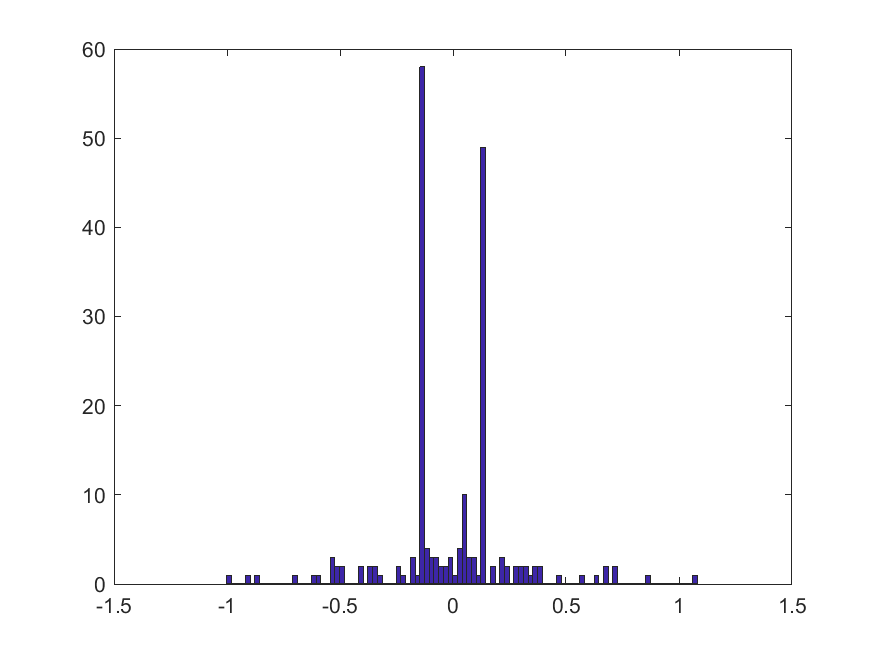
\includegraphics[width=\linewidth]{A_5_4_c.png}
	\caption{Sum of the largest $m/2$ absolute values.}
\end{figure}


(d)\\
Matlab code:

\begin{verbatim}
m = 200;
n = 100;
A = randn(m,n);
b = randn(m,1);
b = b/(1.01*max(abs(b)));

cvx_begin
variable x(n);
minimize sum(max([zeros(m), abs(A * x - b) - 0.2, 2 * abs(A * x - b) - 0.5]))
cvx_end

hist(A*x-b,m/2);
saveas(gcf,'C:/! Convex_Optimization/homework_solutions/part_1/hw5/A_5_4_d.png')
\end{verbatim}

\begin{figure}[H]
	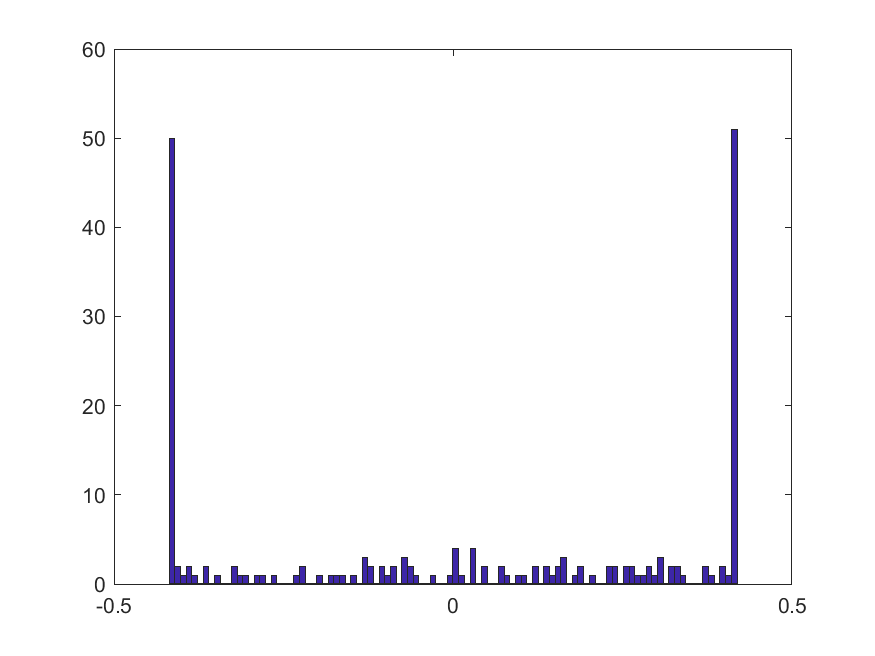
\includegraphics[width=\linewidth]{A_5_4_d.png}
	\caption{A piecewise-linear penalty.}
\end{figure}

(e)\\
Matlab code:

\begin{verbatim}
m = 200;
n = 100;
A = randn(m,n);
b = randn(m,1);
b = b/(1.01*max(abs(b)));

cvx_begin
variable x(n);
minimize sum(huber(A * x - b, 0.2))
cvx_end

hist(A*x-b,m/2);
saveas(gcf,'C:/! Convex_Optimization/homework_solutions/part_1/hw5/A_5_4_e.png');
\end{verbatim}

\begin{figure}[H]
	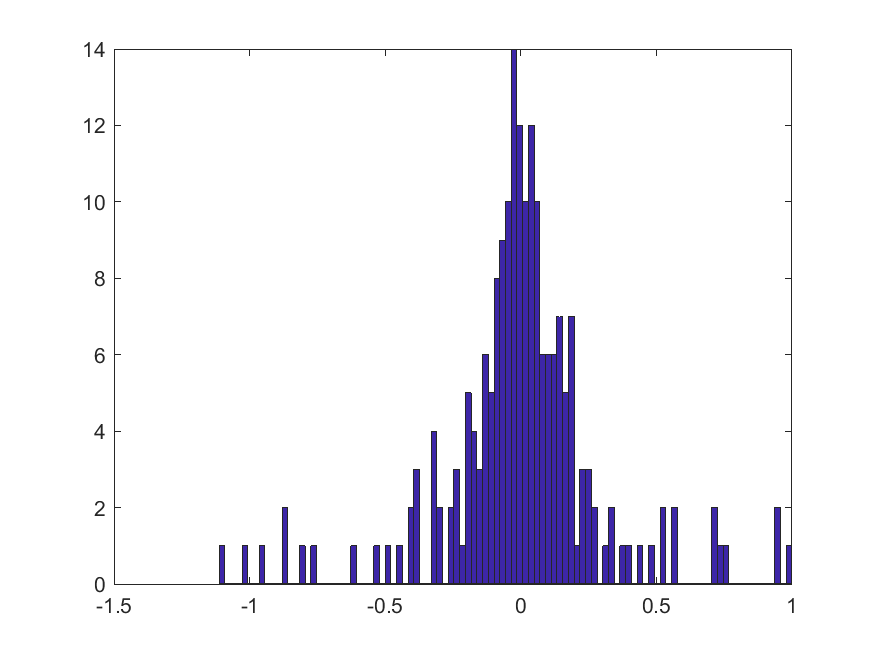
\includegraphics[width=\linewidth]{A_5_4_e.png}
	\caption{Huber penalty.}
\end{figure}


(f)\\
Matlab code:

\begin{verbatim}
m = 200;
n = 100;
A = randn(m,n);
b = randn(m,1);
b = b/(1.01*max(abs(b)));

cvx_begin
variable x(n);
minimize (- geo_mean([1 - A * x + b; 1 + A * x - b]))
cvx_end

hist(A*x-b,m/2);

saveas(gcf,'C:/! Convex_Optimization/homework_solutions/part_1/hw5/A_5_4_f.png')
\end{verbatim}

\begin{figure}[H]
	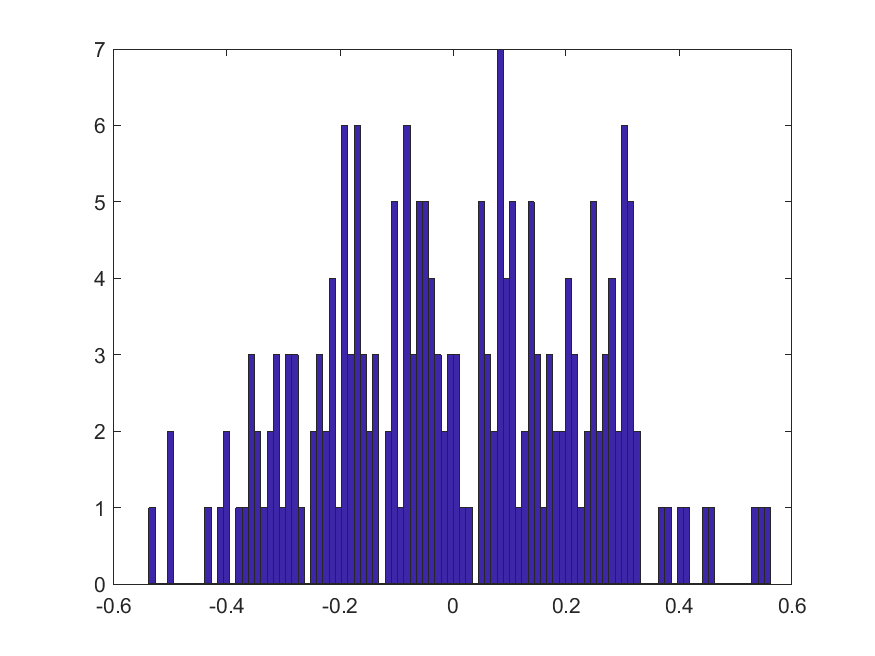
\includegraphics[width=\linewidth]{A_5_4_f.png}
	\caption{Log-barrier penalty.}
\end{figure}

\section*{A12.6} 
Antenna array weight design. We consider an array of $n$ omnidirectional antennas in a plane, at positions
$(x_k, y_k,)$ $k = 1, ..., n.$ 
A unit plane wave with frequency $\omega$ is incident from an angle $\theta$. This incident wave induces in
the kth antenna element a (complex) signal
$exp(i(x_k cos(\theta) + y_k sin(\theta) - \omega t))$ (For
simplicity we assume that the spatial units are normalized so that the wave number is one, i.e., the
wavelength is $\lambda = 2 \pi.$) The baseband signals of the n antennas are combined linearly to form the output of the antenna array 
\begin{align*}
G(\theta) & = \sum_{k = 1}^n \omega_k 
e^{x_k cos(\theta) + y_k sin(\theta)}  \\ 
& = 
\sum_{k = 1}^n (\omega_{re, k} cos(\gamma_k(\theta)) 
- \omega_{im, k} sin(\gamma_k(\theta)) + 
(\omega_{re, k} sin(\gamma_k(\theta)) 
+ \omega_{im, k} cos(\gamma_k(\theta))
\end{align*}
if we define 
$\gamma_k(\theta) = x_k cos(\theta) + y_k sin(\theta)$
The complex weights in the linear combination,
$\omega_k = \omega_{re, k} + i \omega_{im, k}$ are called the antenna array coefficients or shading coefficients, and will be the design variables in the problem. For a given set of weights, the combined output $G(\theta).$ is a function of the angle
of arrival $\theta.$ of the plane wave. The design problem is to select weights $\omega_i$ that achieve a desired
directional pattern $G(\theta).$ We now describe a basic weight design problem. We require unit gain in a target direction
$\theta^{tar}, $ i.e., $G(\theta^{tar}) = 1.$ We want 
$G(\theta)$ small for $|\theta - \theta^{tar}| \geq \Delta.$ This number is called the sidelobe level for the array; our goal is to minimize the sidelobe level. If we achieve a small sidelobe level, then the array is relatively insensitive to signals arriving from directions more than $\Delta$ away from the target direction. This results in the optimization problem:

\begin{align*}
&\text{minimize } && 
\max_{|\theta - \theta^{tar}| \geq \Delta} |G(\theta)|\\
&\text{subject to } 
&& G(\theta^{tar}) = 1
\end{align*}
with $\omega \in C^n$ as variables. \\
The objective function can be approximated by discretizing the angle of arrival with (say) $N$ values (say, uniformly spaced)
$\theta_1, ..., \theta_n$ over an interval $[-\pi, \pi],$ and replacing the objective with 
$$
max\{G(\theta_k) \, | \, |\theta_k - \theta^{tar}| \geq \Delta\}
$$

(a) Formulate the antenna array weight design problem as an SOCP.\\

(b) Solve an instance using CVX, with $n = 40,$ $
\theta^{tar} = 15^{\circ},$ $\Delta = 15^{\circ},$ $N = 400,$ 
and antenna positions generated using:

\begin{verbatim}
rand('state',0);
n = 40;
x = 30 * rand(n,1);
y = 30 * rand(n,1);
\end{verbatim}

Compute the optimal weights and make a plot of $|G(\theta)|$ (on a logarithmic scale) versus $\theta.$ Hint. CVX can directly handle complex variables, and recognizes the modulus \verb|abs(x)| of a
complex number as a convex function of its real and imaginary parts, so you do not need to
explicitly form the SOCP from part (a). Even more compactly, you can use \verb|norm(x,Inf)| with complex argument.

Solution:

The problem can be expressed as the SOCP:

\begin{align*}
&\text{minimize } && 
t \\
&\text{subject to } 
&& ||A_k x ||_2 \leq t, \, k \in \mathcal{I}\\
& && Bx = d \\
\end{align*}
with variables $x,$ $t,$ 
$\mathcal{I} = \{k | \; |\theta - \theta^{tar}| \geq \Delta\}$
and

$$
x = 
\begin{bmatrix}
\omega_{re}\\
\omega_{im}\\
\end{bmatrix}
\in R^{2n}
$$

$$
A_k = 
\begin{bmatrix}
cos(\gamma_1(\theta_k)) & \dots & cos(\gamma_n(\theta_k)) 
& - sin(\gamma_1(\theta_k)) & \dots & - sin(\gamma_n(\theta_k))  \\
cos(\gamma_1(\theta^{tar})) & \dots & cos(\gamma_n(\theta^{tar})) 
& - sin(\gamma_1(\theta^{tar})) & \dots & - sin(\gamma_n(\theta^{tar}))  \\
\end{bmatrix}
$$


$$
B_k = 
\begin{bmatrix}
cos(\gamma_1(\theta^{tar})) & \dots & cos(\gamma_n(\theta^{tar})) 
& - sin(\gamma_1(\theta^{tar})) & \dots & - sin(\gamma_n(\theta^{tar}))  \\
\\
sin(\gamma_1(\theta^{tar})) & \dots & sin(\gamma_n(\theta^{tar})) 
& cos(\gamma_1(\theta^{tar})) & \dots &  cos(\gamma_n(\theta^{tar}))  \\
\end{bmatrix}
$$

$$
d = 
\begin{bmatrix}
1\\0
\end{bmatrix}
$$

the matlab code:

\begin{verbatim}
clear all
rand('state',0);
%N= 10; %400;
%n = 2;%40;
N = 400;
n = 40;
x = 30 * rand(n,1);
y = 30 * rand(n,1);
X = [x'; y'];

beamwidth = 15*pi/180;
theta_tar=15*pi/180;
theta = linspace(theta_tar+beamwidth, 2*pi+theta_tar-beamwidth, N)';
A = exp(i * [cos(theta), sin(theta)] * X);
Atar = exp(i * [cos(theta_tar), sin(theta_tar)] * X);

cvx_begin
variable w(n) complex
minimize(max(abs(A*w)))
subject to
Atar*w == 1;
cvx_end

gamma = zeros(n, N);
for i = 1:n
for j = 1:N
gamma(i, j) = x(i) * cos(theta(j)) + y(i) * sin(theta(j));
end
end
size(gamma)

G = zeros(N, 1);

for i = 1:N
for j = 1:n
omega = w(j);
rw = real(omega);
iw = imag(omega);
g = gamma(j, i);
G(i) = G(i) + complex(rw * cos(g) - iw * sin(g), ...
(rw * sin(g) + iw * cos(g)));
end
end

abs_G = abs(G)


plot(theta, abs(G))
\end{verbatim}

Something wrong with this task here

\end{document}

